% ==========================================================
% Póster académico A1 horizontal · 3 columnas
% Maestría en Inteligencia Artificial Aplicada · Equipo 1
% Basado en poster_plantilla.tex (encabezado, colores, fuentes y tamaños de la plantilla).
% Compilación: latexmk -pdf poster_proyecto.tex
% ==========================================================
\documentclass[10pt]{article}

\usepackage{iftex}
\usepackage[a1paper,landscape,margin=1.5cm]{geometry}
\usepackage[spanish,es-noshorthands]{babel}
\usepackage{xcolor}
\usepackage{graphicx}
\usepackage{tikz}
\usetikzlibrary{arrows.meta,positioning,calc}
\usepackage[most]{tcolorbox}
\usepackage{enumitem}
\usepackage{booktabs}
\usepackage{colortbl}
\usepackage{microtype}

% ---------------------- TIPOGRAFÍA -------------------------
\ifTUTeX
  \usepackage{fontspec}
  \IfFontExistsTF{Instrument Serif}%
    {\newfontfamily\serif{Instrument Serif}}%
    {\newfontfamily\serif{TeX Gyre Pagella}}
\else
  \usepackage[utf8]{inputenc}
  \usepackage[T1]{fontenc}
  \usepackage{lmodern}
  \usepackage[scaled=0.95]{helvet}
  \newcommand{\serif}{\fontfamily{bch}\selectfont}
\fi

\pagestyle{empty}
\setlength{\parindent}{0pt}
\setlength{\parskip}{0.4em}

% ---------------------- PALETA -----------------------------
\definecolor{olive}{HTML}{9AA542}
\definecolor{olivedark}{HTML}{1B2208}
\definecolor{olivelink}{HTML}{6B7A1F}
\definecolor{olivesoft}{HTML}{E4E8C7}
\definecolor{ink}{HTML}{1A1A10}
\definecolor{muted}{HTML}{6B6B5E}
\definecolor{pagebg}{HTML}{FFFFFF}

\pagecolor{pagebg}
\color{ink}

% ---------------------- DATOS DEL PÓSTER -------------------
\newcommand{\programa}{Maestría en Inteligencia Artificial Aplicada}
\newcommand{\tituloA}{Aprendizaje autosupervisado con Contrastive Predictive Coding}
\newcommand{\tituloB}{para reconocer actividades de manejo manual de cargas}
\newcommand{\autores}{Isaura Yutsil Flores Escamilla\quad Paola Alejandra León Guarneros\quad Dylan Ulises Quiroz Hernández}
\newcommand{\asesor}{Dr. Gerardo Jesús Camacho González}
\newcommand{\fecha}{Noviembre 2026}

\newcommand{\logoizq}{
\includegraphics[height=3.3cm]{logo.jpeg}}
\newcommand{\logoder}{
\includegraphics[height=3.3cm]{logo_der.png}}

% ---------------------- ESTILOS ----------------------------
\newcommand{\seccion}[1]{%
  \begin{tcolorbox}[colback=olive,colframe=olive,arc=0pt,
    boxrule=0pt,left=8pt,top=3pt,bottom=4pt,width=\linewidth]
    {\serif\color{white}\fontsize{30}{36}\selectfont #1}
  \end{tcolorbox}\vspace{-0.3em}}

\newcommand{\cuerpo}{\fontsize{24}{31}\selectfont}
\newcommand{\pie}[1]{{\sffamily\fontsize{18}{22}\selectfont\color{muted}#1}}

\newcommand{\circulo}[1]{%
  \tikz\node[circle,fill=olivesoft,minimum size=6cm,align=center,
    text width=5cm,text=olivedark,
    font=\sffamily\bfseries\fontsize{19}{23}\selectfont]{#1};}

% Tarjeta de cifra: \cifra{ancho}{valor}{descripción}
\newcommand{\cifra}[3]{%
  \begin{minipage}[t]{#1}
  \begin{tcolorbox}[colback=olivesoft,colframe=olivesoft,arc=4pt,boxrule=0pt,
    width=\linewidth,left=6pt,right=6pt,top=6pt,bottom=6pt,halign=center,valign=center,height=4.6cm]
    {\serif\fontsize{48}{52}\selectfont\color{olivedark}#2}\\[0.15em]
    {\sffamily\fontsize{18}{22}\selectfont\color{ink}#3}
  \end{tcolorbox}
  \end{minipage}}

% Actividad: \act{código}{nombre}
\newcommand{\act}[2]{%
  \tikz\node[draw=olive,line width=1.5pt,rounded corners=4pt,fill=white,minimum width=5.55cm,
    minimum height=2.1cm,align=center,inner sep=4pt]
    {{\sffamily\bfseries\fontsize{24}{26}\selectfont\color{olivelink}#1}\\[2pt]
     {\sffamily\fontsize{16}{19}\selectfont\color{ink}#2}};}

\newlength{\hdrh}\setlength{\hdrh}{9cm}
\newlength{\colh}
\setlength{\colh}{\dimexpr\textheight-\hdrh-6cm\relax}

% ======================================================
\begin{document}

% ---------------------- ENCABEZADO ------------------------
\noindent\parbox[t][\hdrh][c]{\linewidth}{%
\begin{minipage}[c]{0.145\linewidth}
  \raggedright\logoizq
\end{minipage}%
\begin{minipage}[c]{0.71\linewidth}
  \centering
  {\serif\fontsize{58}{65}\selectfont\color{olivedark}%
   \tituloA\\\tituloB\par}
  \vspace{0.5em}
  {\sffamily\bfseries\fontsize{30}{36}\selectfont\color{olivelink}\programa\par}
  \vspace{0.3em}
  {\fontsize{26}{32}\selectfont\color{ink}\autores\par}
  {\fontsize{22}{28}\selectfont\color{muted}Asesor: \asesor\ \textperiodcentered\ \fecha\par}
\end{minipage}%
\begin{minipage}[c]{0.145\linewidth}
  \raggedleft\logoder
\end{minipage}}

\vspace{0.4cm}
{\color{olive}\rule{\linewidth}{2.5pt}}
\vspace{0.6cm}

% ---------------------- COLUMNAS --------------------------
\noindent
\begin{minipage}[t][\colh][s]{0.30\linewidth}\cuerpo\vspace{0pt}
% ===== COLUMNA IZQUIERDA: problema y datos =====

\seccion{¿Por qué reconocer actividades?}
Manejar cargas a mano es una de las tareas más asociadas con \textbf{lesiones musculoesqueléticas}. Para detectar los movimientos lesivos, primero hay que saber \textbf{qué} hace el trabajador y \textbf{cuándo}.

\begin{center}
\act{N}{Postura neutral}\hspace{0.15cm}\act{LF}{Levantar del piso}\hspace{0.15cm}\act{K}{Mantener la carga}\hspace{0.15cm}\act{W}{Caminar con carga}\\[0.2cm]
\act{LT}{Levantar de mesa}\hspace{0.15cm}\act{PT}{Colocar en mesa}\hspace{0.15cm}\act{PF}{Colocar en piso}
\end{center}

\begin{minipage}[c]{0.40\linewidth}
  \centering
  \begin{tikzpicture}
    \fill[olivesoft] (0,0) arc (180:0:4.5 and 4.5) -- (6,0) arc (0:180:3 and 3) -- cycle;
    \node[font=\serif\fontsize{64}{68}\selectfont,text=olivedark] at (4.5,1.1) {600};
  \end{tikzpicture}
\end{minipage}\hfill
\begin{minipage}[c]{0.58\linewidth}
  segmentos marcados \textbf{a mano} por cada persona grabada. Anotar es lento y costoso.
\end{minipage}

\vspace{0.3em}
\begin{tcolorbox}[colback=olivesoft,colframe=olive,boxrule=2pt,arc=4pt,left=10pt,right=10pt]
\textbf{Pregunta:} ¿un modelo preentrenado \emph{sin etiquetas} iguala al supervisado con personas nuevas y lo supera con \textbf{pocas etiquetas}?
\end{tcolorbox}

\vfill
\seccion{Datos y evaluación}
14 personas · 37 ensayos · cargas de 2 a 12~kg · traje de 17 sensores inerciales y electromiografía (sEMG).
\begin{center}
  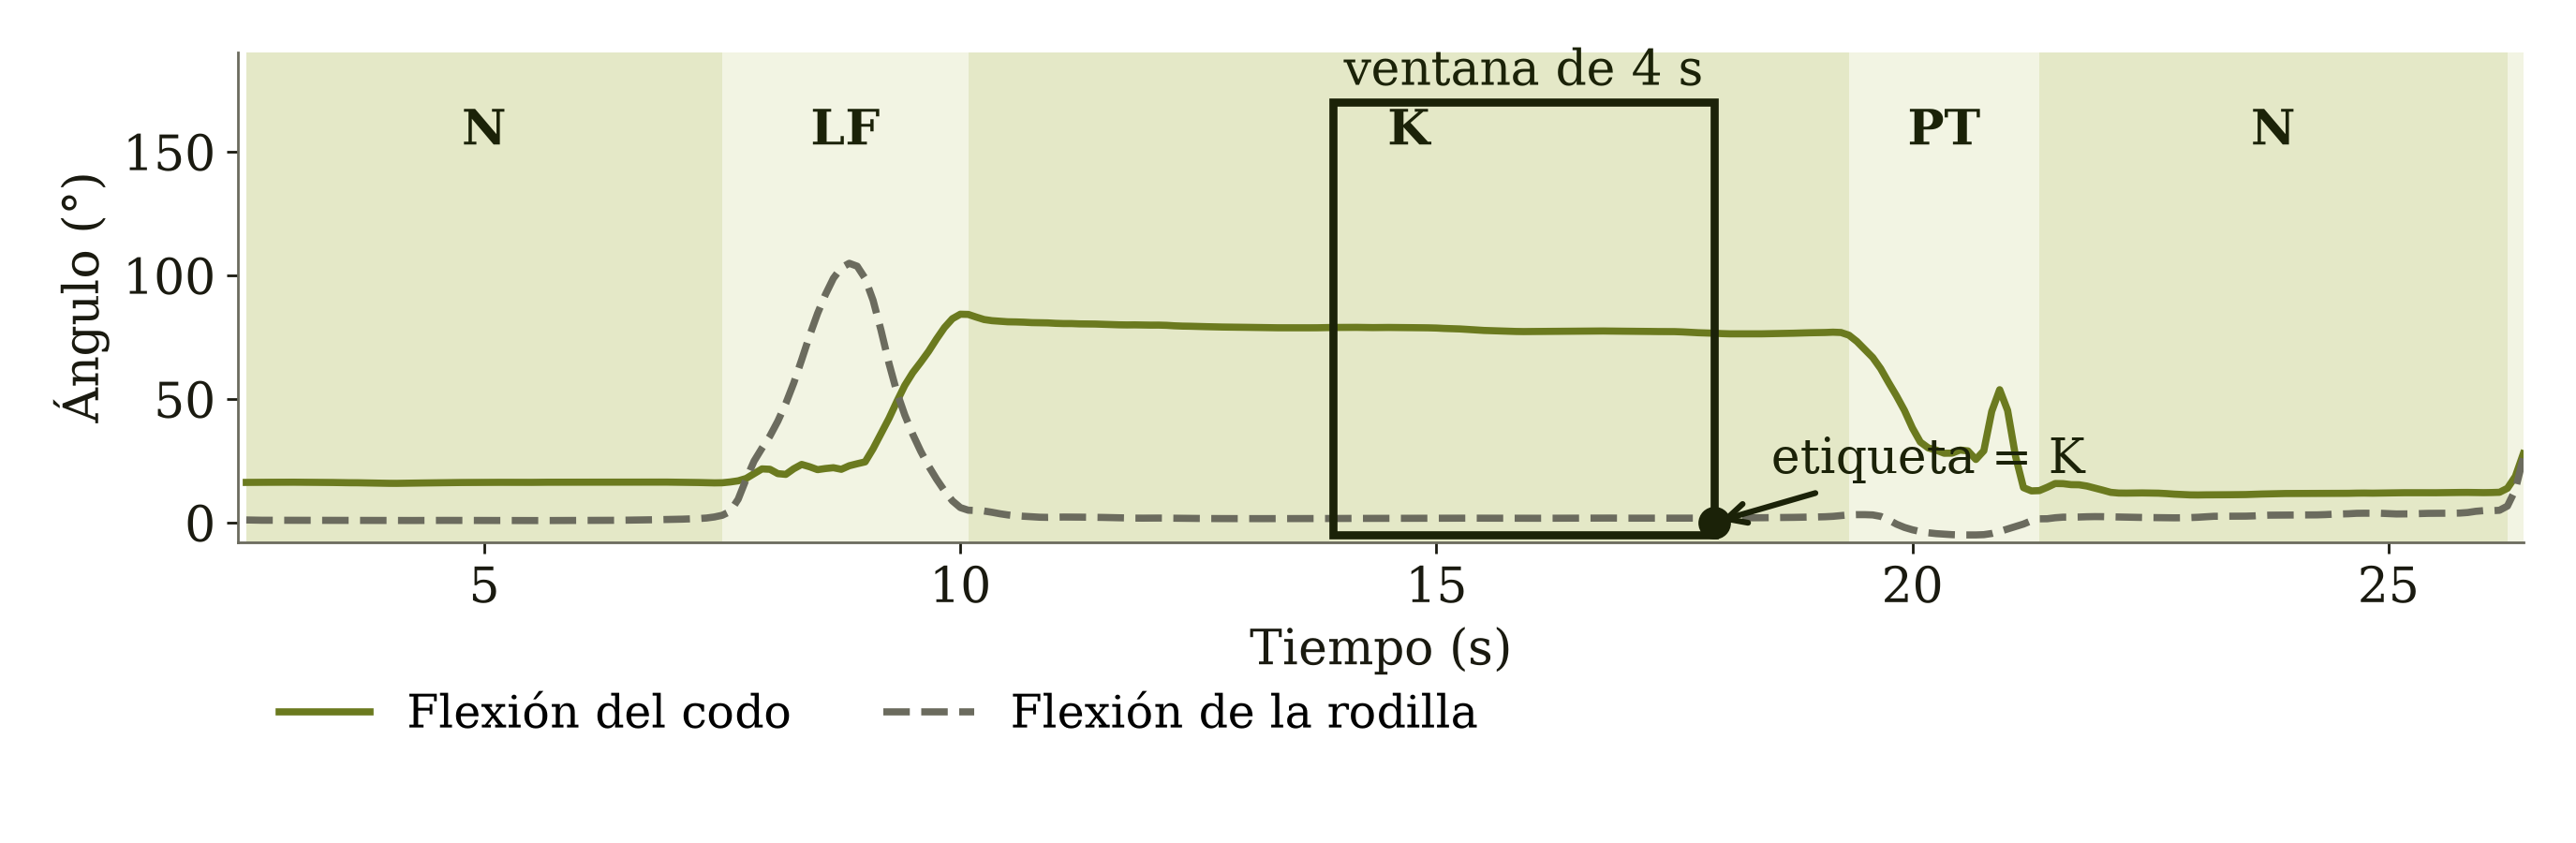
\includegraphics[width=\linewidth]{fig_ventana.png}\\[2pt]
  \pie{Figura 1. Cada ventana de 4 s se etiqueta con la actividad de su último instante.}
\end{center}
Siempre con \textbf{personas nuevas}: 12 rondas dejando una fuera y 2 reservadas para la prueba final.

\vfill
\seccion{Del músculo al movimiento}
\begin{center}
\begin{tikzpicture}[x=15cm,y=0.85cm]
  \foreach \y/\lab/\v/\c in {2.4/sEMG/0.485/muted, 1.2/sEMG + movimiento/0.880/olive, 0/Movimiento/0.885/olivelink}{
    \fill[\c] (0,\y) rectangle (\v,\y+0.85);
    \node[anchor=east,font=\sffamily\fontsize{20}{24}\selectfont] at (0,\y+0.42) {\lab};
    \node[anchor=west,font=\sffamily\bfseries\fontsize{20}{24}\selectfont] at (\v,\y+0.42) {\v};
  }
  \draw[muted,line width=1pt] (0,-0.2) -- (0,3.45);
\end{tikzpicture}\\[2pt]
\pie{Figura 2. F1 macro con cada fuente: sólo el movimiento distingue piso de mesa.}
\end{center}

\end{minipage}\hfill
\begin{minipage}[t][\colh][s]{0.37\linewidth}\cuerpo\vspace{0pt}
% ===== COLUMNA CENTRAL: modelo y hallazgo principal =====

\seccion{El modelo: CPC con red GRU}
\begin{center}
\begin{tikzpicture}[
  font=\sffamily\fontsize{20}{24}\selectfont,
  box/.style={draw=olivelink,line width=2pt,rounded corners=4pt,align=center,minimum height=2.6cm,inner sep=5pt,fill=white},
  pre/.style={box,fill=olivesoft},
  aux/.style={box,dashed,draw=muted,text=muted},
  head/.style={box,fill=olive,text=white,draw=olive},
  arr/.style={-{Stealth[length=6mm]},line width=3pt,color=olivelink}]
  \node[box,text width=4.3cm] (x) {Ventana de 4 s\\ 10 variables};
  \node[pre,right=0.9cm of x,text width=4.3cm] (enc) {Encoder\\ causal};
  \node[pre,right=0.9cm of enc,text width=3.2cm] (gru) {GRU};
  \node[aux,right=1.4cm of gru,yshift=1.75cm,text width=8.6cm,minimum height=2.3cm] (pred) {\textbf{Fase 1 · sin etiquetas}\\ predice el movimiento\\ hasta 1 s adelante};
  \node[head,right=1.4cm of gru,yshift=-1.75cm,text width=8.6cm,minimum height=2.3cm] (cab) {\textbf{Fase 2 · con etiquetas}\\ cabeza lineal $\to$ 7 actividades};
  \draw[arr] (x) -- (enc);
  \draw[arr] (enc) -- (gru);
  \draw[arr,muted] (gru.east) -- ++(0.7,0) |- (pred.west);
  \draw[arr] (gru.east) -- ++(0.7,0) |- (cab.west);
\end{tikzpicture}\\[4pt]
\pie{Figura 3. Aprende sin etiquetas y luego se ajusta con pocas (725 mil parámetros, causal).}
\end{center}

\vfill
\seccion{Bastan 11 de 17 sensores}
\begin{minipage}[c]{0.36\linewidth}
\centering
\begin{tikzpicture}[scale=0.85,
  keep/.style={circle,fill=olivelink,minimum size=0.75cm,inner sep=0pt},
  drop/.style={circle,draw=muted,line width=2pt,fill=white,minimum size=0.75cm,inner sep=0pt},
  bone/.style={line width=7pt,color=olivesoft,line cap=round}]
  % esqueleto
  \draw[bone] (0,7.3) -- (0,3.6);
  \draw[bone] (-1.3,6.2) -- (1.3,6.2);
  \draw[bone] (-1.3,6.2) -- (-1.8,4.6) -- (-2.1,3.1);
  \draw[bone] (1.3,6.2) -- (1.8,4.6) -- (2.1,3.1);
  \draw[bone] (-0.7,3.6) -- (0.7,3.6);
  \draw[bone] (-0.7,3.6) -- (-0.8,1.8) -- (-0.85,0.1);
  \draw[bone] (0.7,3.6) -- (0.8,1.8) -- (0.85,0.1);
  \fill[olivesoft] (0,8.1) circle (0.75);
  % sensores que se quitan
  \node[drop] at (0,8.1) {}; \node[drop] at (0,6.6) {};
  \node[drop] at (-1.1,6.2) {}; \node[drop] at (1.1,6.2) {};
  \node[drop] at (-1.1,-0.2) {}; \node[drop] at (1.1,-0.2) {};
  % sensores que se conservan
  \node[keep] at (0,3.6) {};
  \foreach \s in {-1,1}{
    \node[keep] at (\s*1.6,5.3) {}; \node[keep] at (\s*2.0,3.8) {}; \node[keep] at (\s*2.1,2.9) {};
    \node[keep] at (\s*0.75,2.6) {}; \node[keep] at (\s*0.82,1.0) {};
  }
\end{tikzpicture}
\end{minipage}\hfill
\begin{minipage}[c]{0.60\linewidth}
\tikz\node[circle,fill=olivelink,minimum size=0.75cm]{}; se conservan (11): pelvis, brazos, antebrazos, manos, muslos y piernas.\par
\tikz\node[circle,draw=muted,line width=2pt,minimum size=0.75cm]{}; se quitan (6): cabeza, tronco alto, hombros y pies.\par
\vspace{0.3em}
F1 de \textbf{0.873} frente a 0.878 con los 17: \textbf{sin diferencia significativa}.
\end{minipage}

\vfill
\seccion{Hallazgo principal: con pocas etiquetas, CPC gana}
\begin{center}
  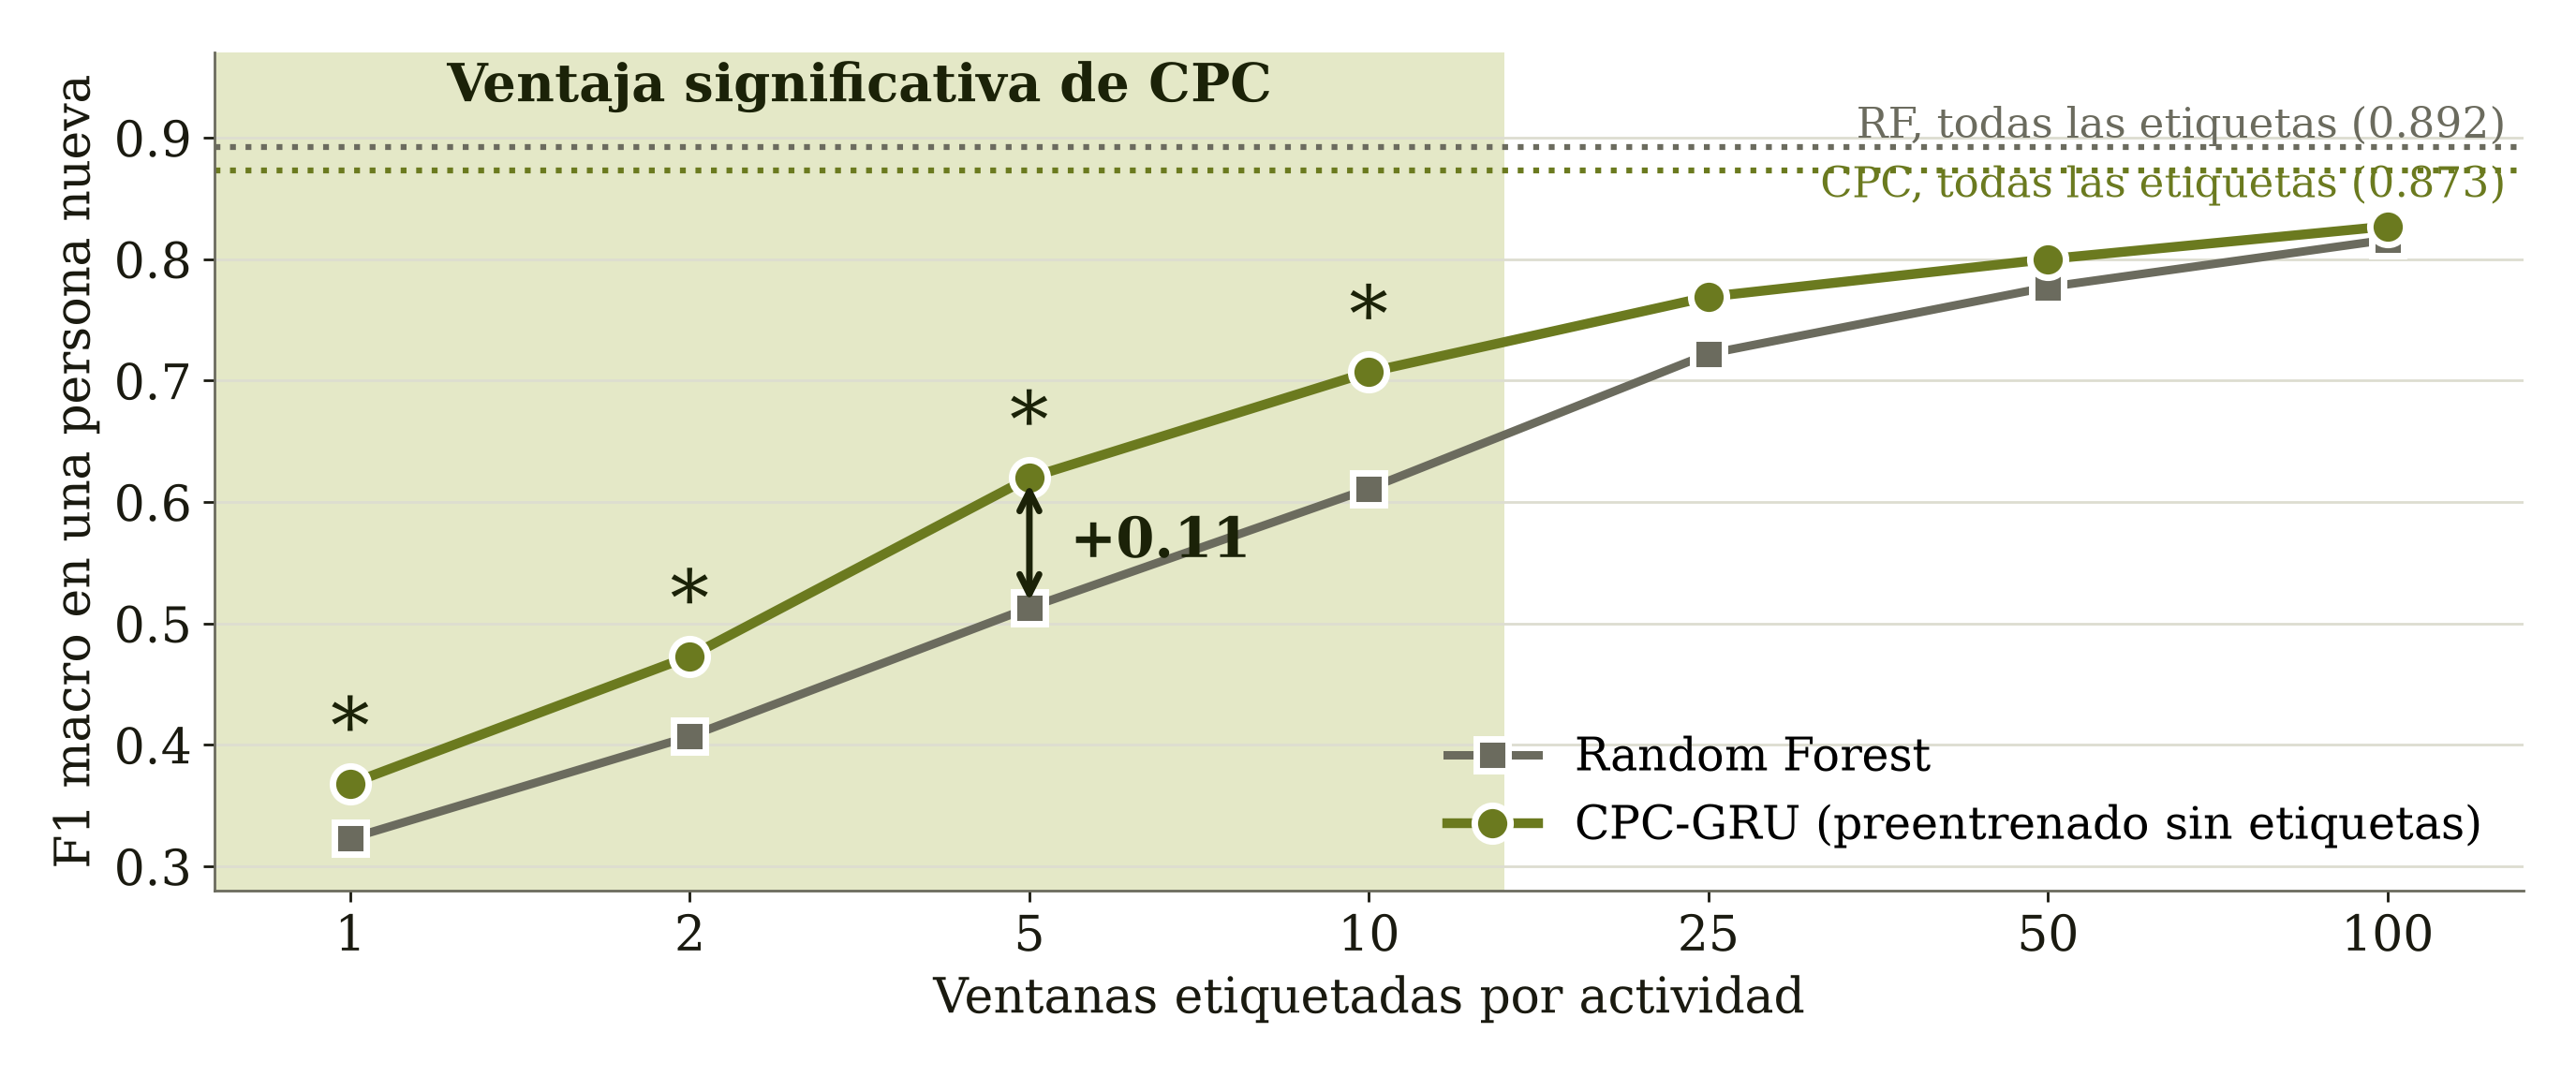
\includegraphics[width=\linewidth]{fig_pocas.png}\\[2pt]
  \pie{Figura 4. F1 macro en una persona nueva (* $p < 0.05$, Wilcoxon con corrección de Holm).}
\end{center}
\noindent
\cifra{0.32\linewidth}{+0.11}{F1 sobre el Random Forest\\ con 5 ventanas por actividad}\hfill
\cifra{0.32\linewidth}{2.2$\times$}{menos etiquetas para\\ el mismo desempeño}\hfill
\cifra{0.32\linewidth}{11--12}{de 12 personas mejoran\\ con $\le 10$ ventanas}

\end{minipage}\hfill
\begin{minipage}[t][\colh][s]{0.30\linewidth}\cuerpo\vspace{0pt}
% ===== COLUMNA DERECHA: desempeño, conclusiones y aplicación =====

\seccion{¿Qué tan bien funciona?}

\begin{center}
\pie{Tabla 1. F1 macro con todas las etiquetas.}

\vspace{0.3em}
\fontsize{20}{26}\selectfont
\renewcommand{\arraystretch}{1.35}
\arrayrulecolor{olivedark}
\begin{tabular}{lcc}
  \toprule
  \textbf{Modelo} & \textbf{Personas nuevas} & \textbf{Prueba final} \\
  \midrule
  Random Forest (10 var.) & 0.892 & 0.885 · 0.906 \\
  \textbf{CPC-GRU (10 var.)} & \textbf{0.873} & \textbf{0.884 · 0.898} \\
  BiLSTM (Bassani et al., 2025) & 0.903$^{*}$ & --- \\
  \bottomrule
\end{tabular}\\[3pt]
\pie{$^{*}$ Una sola persona y otro protocolo; en una réplica, CPC-GRU obtuvo 0.910.}
\end{center}
Con todas las etiquetas, CPC queda \textbf{cerca} del modelo supervisado. Los errores están en las fronteras entre actividades; piso y mesa casi no se confunden ($\le 4$\,\%).

\vfill
\seccion{Conclusiones clave}
\begin{center}
  \circulo{El movimiento\\supera a\\la sEMG}\hspace{0.2cm}
  \circulo{Bastan\\11 sensores}\hspace{0.2cm}
  \circulo{Con pocas\\etiquetas,\\CPC gana}
\end{center}
CPC conviene cuando hay \textbf{mucho movimiento grabado y pocas anotaciones}: es el caso de una persona, tarea o entorno nuevos.

\vfill
\seccion{Hacia la aplicación}
\begin{center}
\begin{tikzpicture}[
  paso/.style={draw=olivelink,line width=2pt,rounded corners=4pt,fill=olivesoft,align=center,
    font=\sffamily\bfseries\fontsize{19}{23}\selectfont,text width=5cm,minimum height=3cm},
  arr/.style={-{Stealth[length=6mm]},line width=4pt,color=olive}]
  \node[paso] (a) at (0,0) {11 sensores\\ inerciales};
  \node[paso] (b) at (7.4,0) {CPC-GRU\\ cada 0.5 s};
  \node[paso] (c) at (14.8,0) {Línea de tiempo\\ de actividades};
  \draw[arr] (a.east) -- (b.west);
  \draw[arr] (b.east) -- (c.west);
\end{tikzpicture}
\end{center}
Siguiente paso: validar con trabajadores y un kit real de 11 sensores, y pasar de actividades a \textbf{movimientos lesivos}.

\vfill
\seccion{Referencias}
{\fontsize{18}{23}\selectfont
\begin{itemize}[leftmargin=1.2em,itemsep=0.2em]
  \item Bassani, G., Avizzano, C. A., y Filippeschi, A. (2025). Deep learning algorithms for human activity recognition in manual material handling tasks. \emph{Sensors, 25}(21), 6705.
  \item Bassani, G., Filippeschi, A., y Avizzano, C. A. (2021). \emph{Manual material handling dataset for biomechanical and ergonomics analysis} [Conjunto de datos]. Zenodo.
  \item Haresamudram, H., Essa, I., y Plötz, T. (2021). Contrastive predictive coding for human activity recognition. \emph{Proc.\ ACM IMWUT, 5}(2), 1--26.
  \item van den Oord, A., Li, Y., y Vinyals, O. (2018). \emph{Representation learning with contrastive predictive coding}. arXiv:1807.03748.
\end{itemize}}

\end{minipage}

\vfill
% ---------------------- DECLARACIÓN DE IA ------------------
{\color{olive}\rule{\linewidth}{2.5pt}}
\vspace{0.3cm}

\noindent
{\fontsize{18}{23}\selectfont\color{ink}
{\serif\color{olivedark}\fontsize{22}{28}\selectfont Declaración de uso de inteligencia artificial.}
Se utilizó Claude Code (Anthropic, 2026) para generar y optimizar el código de los experimentos y para redactar y dar formato a este póster; el equipo definió los experimentos y verificó las cifras.
La responsabilidad final sobre el contenido entregado recae en los autores.\par}

\end{document}
